\section{Data Link Lag}
Datalinklaget er det første lag efter det fysiske. Det yder services til transportlaget og modtager services fra det fysiske lag.
    Det afsendende datalinklag skal modtage payloads fra transportlaget, og har ansvaret for at pakke disse ned i et format, der tillader det modtagende lag at genkende og finde fejl i den transmitterede data.
    Det modtagende datalinklag skal modtage bitstrøm fra sit fysiske lag, og er ansvarlig for genkendelsen og opdelingen af disse i de originale datapakker, som afsenderen gav til sit fysiske lag. Herefter skal det originale payload fra afsenderens transportlag verificeres og udvindes, således at det kan gives videre til det modtagende transportlag.

\subsection{Afsender}
For at facilitere den logiske forbindelse mellem de afsendende- og modtagende datalinklag, er det relevant at beslutte sig for et pakkeformat, som begge sider kender til. Der er her fokus på overvejelser omkring pakkernes størrelse, udformning og afgrænsning, samt hvilken redundant information der tilføjes, for at opnå den førnævnte funktionalitet.

\begin{figure}[h]
\centering
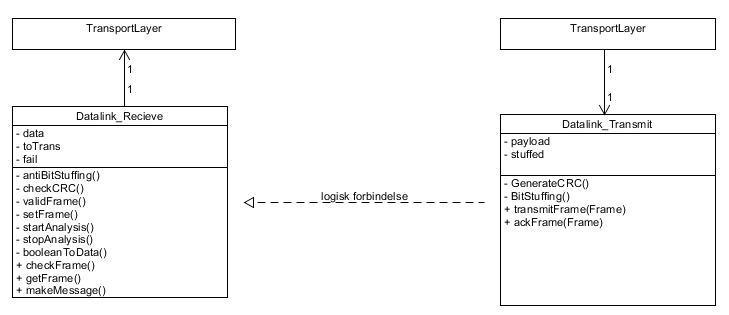
\includegraphics[scale=0.7]{Billeder/DataLinkLogical.PNG}
\caption{Her ses et uddrag fra designklassediagrammet, som viser den logiske forbindelse mellem to datalinklag}
\label{fig:DataLinkLogical}
\end{figure}

\subsubsection{Bit- eller karakter-orienteret protokol}
Datalinklaget skal behandle information som en serie af enten bits eller bytes. Projektets primære mål om at oprette en forbindelse mellem to klienter kan opfyldes med begge protokoltyper, hvor det er relevant at vurdere sekundære ting såsom protokollernes effekt på transmissionshastighed.
I en byte-orienteret protokol behandles data som en streng af karakterer. I denne type kan redundant information kun tilføjes som hele bytes.
En bit-orienteret protokol behandler data som en strøm af bits. Her kan redundant information tilføjes bitvist. 
    Den byte-orienterede protokol virkede i første omgang som det bedste valg, da det primære mål for projektet er at skabe en chat-klient, hvor der udveksles tekst-beskeder, som er lette at pakke ned i en byte-orienteret frame. Samme resultat kan imidlertid også opnås med en bit-orienteret protokol, men denne er i tilgift mere kompatibel med andre datatyper, og er samtidig også mere kompakt når det kommer til tilføjelse af redundant information, hvilket giver et kortere pakkeformat og en hurtigere transmission. I tilgift blev det også fundet lettere at arbejde med bits, da en CRC-division skulle foretages. Af disse årsager blev en bit-orienteret protokol valgt.

\subsubsection{Fast eller variabel framelængde}
Datalinklagets datapakker kan enten have en fast defineret længde, eller en variabel længde.
Vælges en fast længde på alle pakker, bliver pakkernes længde en afgrænsning i sig selv - og det er således ikke nødvendigt at indsætte start- og stopflag. Hvis en pakke er mindre end den definerede længde, er det nødvendigt at tilføje yderligere, redundant information for at opfylde kravet.
Er pakkernes længde variabel, er det nødvendig at indsætte flag i begyndelsen og slutningen af hver frame. Hvis disse bitmønstre indgår i datastrømmen, er det nødvendigt at indsætte redundant information i afsenderen, så ikke bliver misfortolket af det modtagende datalinklag.
Et af projektets primære mål er udviklingen af en chat-klient. Chat-beskeder er af naturlige årsager af meget varierende længde. Af denne årsag er det svært at finde en uniform pakke-længde, der minimerer spild i datatransmissionen. Derfor blev frames med variabel længde valgt.

\subsubsection{Pakkeindhold}
Efter præmisserne for pakkernes opbygning var fastsat, skulle deres indhold fastsættes. 

\begin{figure}[h]
\centering
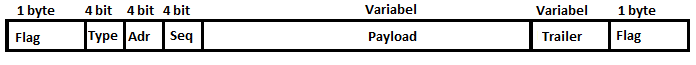
\includegraphics[scale=0.8]{Billeder/DataLinkFrame.PNG}
\caption{Her ses udformningen af en pakke på datalinklagets niveau}
\label{fig:DataLinkFrame}
\end{figure}

Flag: Pakkerne af variabel størrelse markeres gennem hhv. start- og stopflag. Hvis disse flag indgår i dataens bitmønster, er det nødvendigt at tilføje bits i data-link lagets afsender, så disse ikke bliver forvekslet med begyndelsen eller afslutningen på en frame. Disse indsatte bits skal ligeledes fjernes i afsenderen. 

\textbf{Type:} Da der ønskes to typer beskeder i implementeringen af en stop-and-wait protokol (XXXX Reference til valget af stop-and-wait?? Dette valg skal gerne begrundes under programopbygningen Connection-oriented = ack), er det nødvendigt med et type-felt. Dette denoterer pakken som enten værende en kvitterings- eller datapakke.
\textbf{Adresse:} Ét af projektets sekundære mål, er muligheden for kommunikation mellem mere end to klienter. For at muliggøre dette indsættes et adressefelt, som skal indeholde modtagerens adresse. Dette felt kan desuden benyttes af en afsender, til at sortere egne pakker væk, såfremt disse skulle blive opfanget.
\textbf{Sekvensnummer:} Med henblik på at holde de enkelte pakker i en begrænset længde, skal længere beskeder opdeles i flere pakker, i hvilken forbindelse det er relevant at operere med et sekvensnummer.
\textbf{Trailer:} For at hindre korrupt data i at nå de øvre lag, skal der implementeres en form for fejl-kontrol på datalinklaget. Det blev besluttet at implementere et CRC, da dette er en del af IP / TCP standarden, hvilket protokollen er inspireret af. Det er samtidig er en simpel og effektiv måde at detektere fejl.
Der er implementeret CRC af varierende størrelser. Dataordet, som består af pakkens header samt payload, får tilføjet nogle redundante bit, og divideres igennem med et generatorpolynomie. Resten fra denne division påsættes til sidst enden af det originale dataord.	Valget af denne CRC-generator påvirker længden af fejl der med garanti bliver fundet, samt sandsynligheden for at detektere burst-fejl med højere længde end generatorpolynomiet.

Et CRC8 detekterer alle burst-fejl med en længde under 8. I dette tilfælde kan sandsynligheden for at detektere fejl af højere længde findes som $1-1/2^8 = 99,61\%$
Et CRC16 detekterer alle burst-fejl med en længde under 16. Sandsynligheden for at detektere længere fejl findes som $1-½^16 = 99,9999\%.$
    Der blev valgt ikke at fokusere på manuel dimensionering af en generator. Istedet benyttedes et standardpolynomie, der med garanti opfylder kravene opfylder kravene for gode polynomier.

\subsubsection{Cpp implementering}
Da pakkens indhold og udformning var blevet fastsat, skulle denne opbygning implementeres i Cpp-klassen “Datalink-transmit”

\textbf{Beholder-format}
I C++ implementeringen af afsenderen, var det oplagt at arbejde med et beholder-format, med beholdere til at indeholde pakkernes forskellige data-elementer.
I denne forbindelse blev der overvejet hhv. arrays og vector-biblioteket i C++. 
Arrays er som udgangspunkt statisk allokerede beholdere.
Vectorer er dynamisk allokerede, og har indbygget funktionalitet til bla. automatisk ændring af størrelse, samt måling af længde. “Bag facaden”, er dette implementeret igennem allokering af mere end den nødvendige hukommelse, og kopiering af vector-indholdet til nye placeringer, når den tilsidesatte hukommelse ikke længere er tilstrækkelig. 
Valget faldt i sidste ende på vectors. De indbyggede funktionaliteter i vector-biblioteket er nyttige, da det ikke på forhånd er nødvendigt at deklarere længden på beholderen, og disse bit-for-bit kan opbygges eller modificeres. Dette er idéelt når der vælges en protokol med variable størrelser på pakker. Såfremt der var blevet valgt en fast størrelse på pakkerne, kunne arrays benyttes istedet, og der kunne spares nogle system-operationer.

\textbf{Vigtigste metoder}
Afsenderen arbejder med følgende metoder, der implementerer de tidligere nævnte funktionaliteter og principper.
generateCRC()
bitStuffing()
Hjælpemetoder der tilføjer hhv. CRC og bitStuffing til en vector.
transmitFrame()
Opbygger en pakke bit-for-bit i en vector, og sender denne vector videre til sit fysiske lag.


\subsection{Modtager}
Modtager en bitstreng fra det fysiske lag. Leder efter flag i bitstrengen, og sender frames op til transportlaget. 